\documentclass[11pt]{article}
\usepackage{geometry}
\geometry{margin=100pt}
\usepackage[utf8]{inputenc}
\usepackage{graphicx}
\usepackage{epstopdf}
\usepackage{titlesec}
\usepackage{biblatex}
\usepackage{float}
\usepackage{pdfpages}
\newcommand{\horrule}[1]{\rule{\linewidth}{#1}} 
\titleformat{\chapter}{\large\bfseries\centering}{}{0pt}{\huge}
\begin{document}
%opening

\title{
	\vspace{-30mm}
	{\LARGE Machnine Learning (PDEEC0049)\\ \Large Homework 1 }\\[80mm]
    {
\includegraphics[scale=0.1]{feup-logo}}\\[50mm]
}
\author{Shashank Gaur - UP201309443\\}
\date{October 19, 2014}
\maketitle
\newpage
\section{Problem 1}
\subsection{Question 1}

\begin{figure}[H]
	\centering
	\includegraphics[scale=0.25]{{plot_trainingset}}
	\caption{training set plot}
\end{figure}

\subsection{Question 2}
Mean of X1 dataset [[ 5.00287044  5.97561985]] \\
Mean of X2 dataset [[ 1.98304658  2.00294107]] \\
Mean of X3 dataset [[ 0.01535631  6.01730798]] \\
Cov of X1 dataset [[ 1.01607307  0.0134706 ]
 					[ 0.0134706   1.01565189]]\\ 
Cov of X2 dataset [[ 1.01827835  0.00437229]
					[ 0.00437229  1.00719966]]\\ 
Cov of X3 dataset [[ 1.9229381   0.98014156]
					[ 0.98014156  0.98815543]]\\


\subsection{Question 3}
\begin{figure}[H]
	\centering
	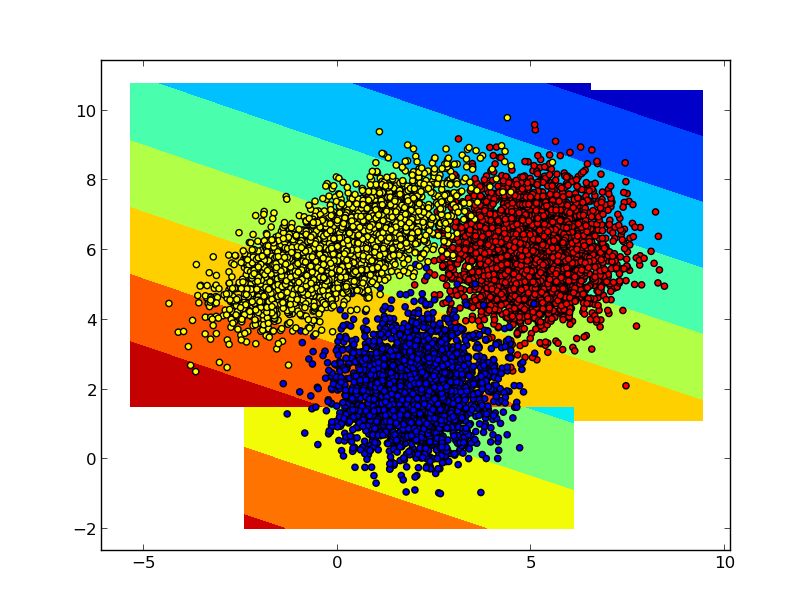
\includegraphics[scale=0.25]{boundry}
	\caption{boundry for classification with contours}
\end{figure}
\newpage

\begin{figure}[H]
	\centering
	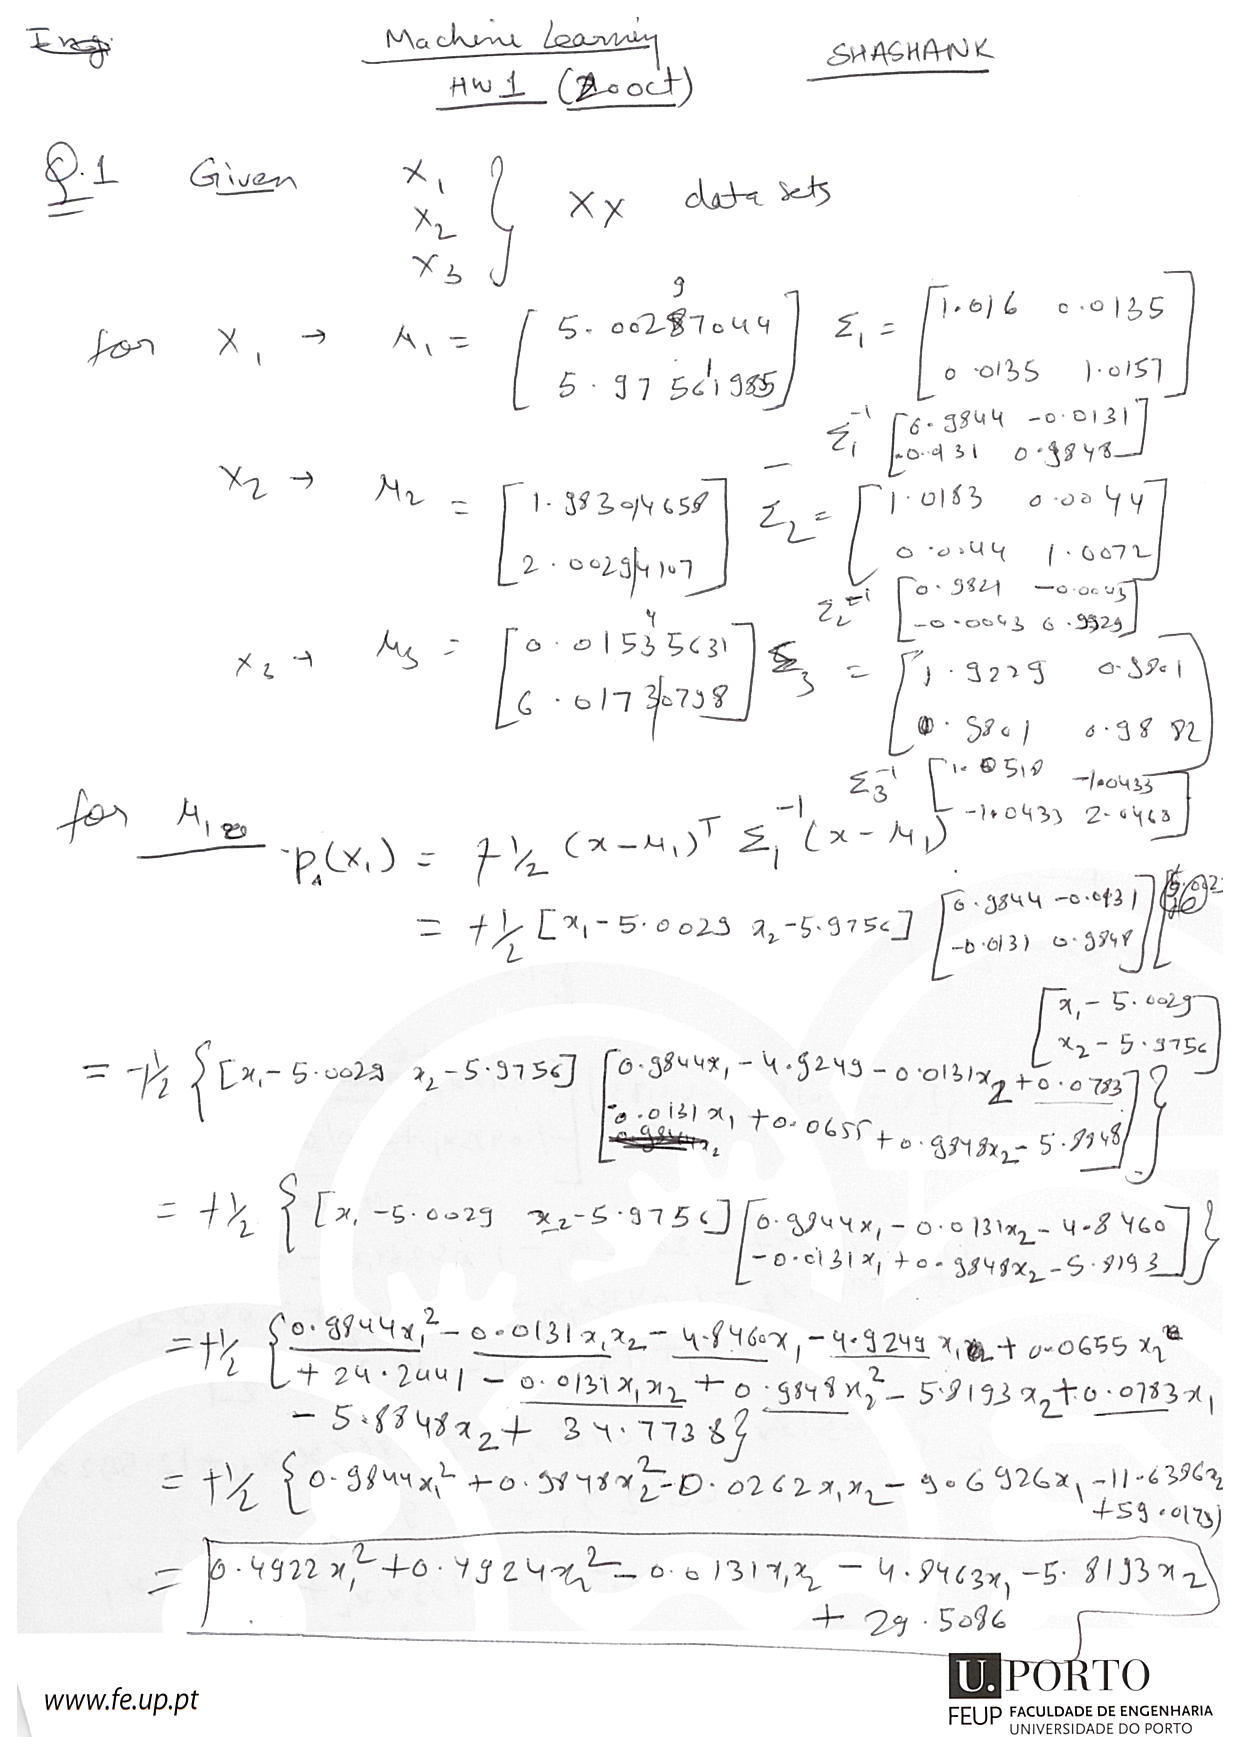
\includegraphics[page=1,scale=0.65]{scans}
\end{figure}
\newpage

\newpage

\begin{figure}[H]
	\centering
	\includegraphics[page=2,scale=0.65]{scans}
\end{figure}
\newpage

\newpage

\begin{figure}[H]
	\centering
	\includegraphics[page=3,scale=0.65]{scans}
\end{figure}
\newpage
\subsection{Question 4}

\begin{figure}[H]
	\centering
	\includegraphics[scale=0.25]{{plot_XX}}
	\caption{training set plot}
\end{figure}
\section{Problem 2}
\subsection{Question 1}

\begin{figure}[H]
	\centering
	\includegraphics[scale=0.5]{{final}}
	\caption{PDF and Decision function in the left plot}
\end{figure}
Probability Density Function\\
For A = exp(-x)\\
For B = (sqrt(2*pi))*exp(-(y-2)**2)\\
Decision Functions\\
For A = 0.4*exp(-x)\\
For B = 0.6*(sqrt(2*pi))*exp(-(y-2)**2)\\
\subsection{Question 2}

With 0.30 probability of error, for x = 1 the class would be B with 0.55 probability. Probability fo Class A would be 0.15.\\
\subsection{Question 3}

\begin{figure}[H]
	\centering
	\includegraphics[scale=0.5]{{min_error}}
	\caption{Minimum error regions in shaded}
\end{figure}

With consideration of Error cost\\
For A = 1.2*0.4*exp(-x)\\
For B = 0.8*0.6*(sqrt(2*pi))*exp(-(y-2)**2)\\
\section{Problem 3}
\begin{figure}[H]
	\centering
	\includegraphics[scale=0.5]{{plot_both}}
	\caption{The plots of both F1(x) and F2(x)}
\end{figure}
\subsection{Question 1}
for F1(x) the value of a and b are 4.98582995951 0
\subsection{Question 2}
for F2(y) the value of c and d are 0.200178803641 0
\subsection{Question 3}
the value of y at x=5 by F1(x) is 24.9291497976\\
the value of y at x=5 by F2(y) is 24.9776695087
\subsection{Question 4}
Preferred model is F1(x)

\end{document}